% Provenance (never printed): 6e geography and cycle 3 sciences (locating a
% place on the globe: parallels, meridians, latitude, longitude; the Earth's
% rotation and time zones); see sources/book1/PROVENANCE.md.
% Book 1, grade 6, chapter 2.
\chapter{Latitude, longitude et fuseaux horaires}\label{ch:g6:latitude-longitude}

La nuit est tombée sur l'\omterm{def:g2:water-on-earth:ocean}{océan}. Sur le pont d'un voilier, en l'an 1750, le
navigateur lève son instrument vers une étoile brillante et mesure sa
hauteur au-dessus de la \omterm{def:g2:water-on-earth:ocean}{mer}. Quelques minutes de travail, et il sait à
quelle distance au nord de l'\omterm{def:g3:continents-and-oceans:equator}{équateur} se trouve le navire. Mais à quelle
distance vers l'est ou vers l'ouest~? Cela, il ne peut pas le dire. Le
problème était si grave qu'en 1714 le Parlement britannique avait promis
un prix important à quiconque trouverait un moyen de la mesurer en \omterm{def:g2:water-on-earth:ocean}{mer}.
Aujourd'hui, le téléphone qui est dans ta poche donne les deux réponses en
une seconde.
% ledger: rmg:15deg-per-hour, rmg:longitude-act-1714

\begin{omfigure}
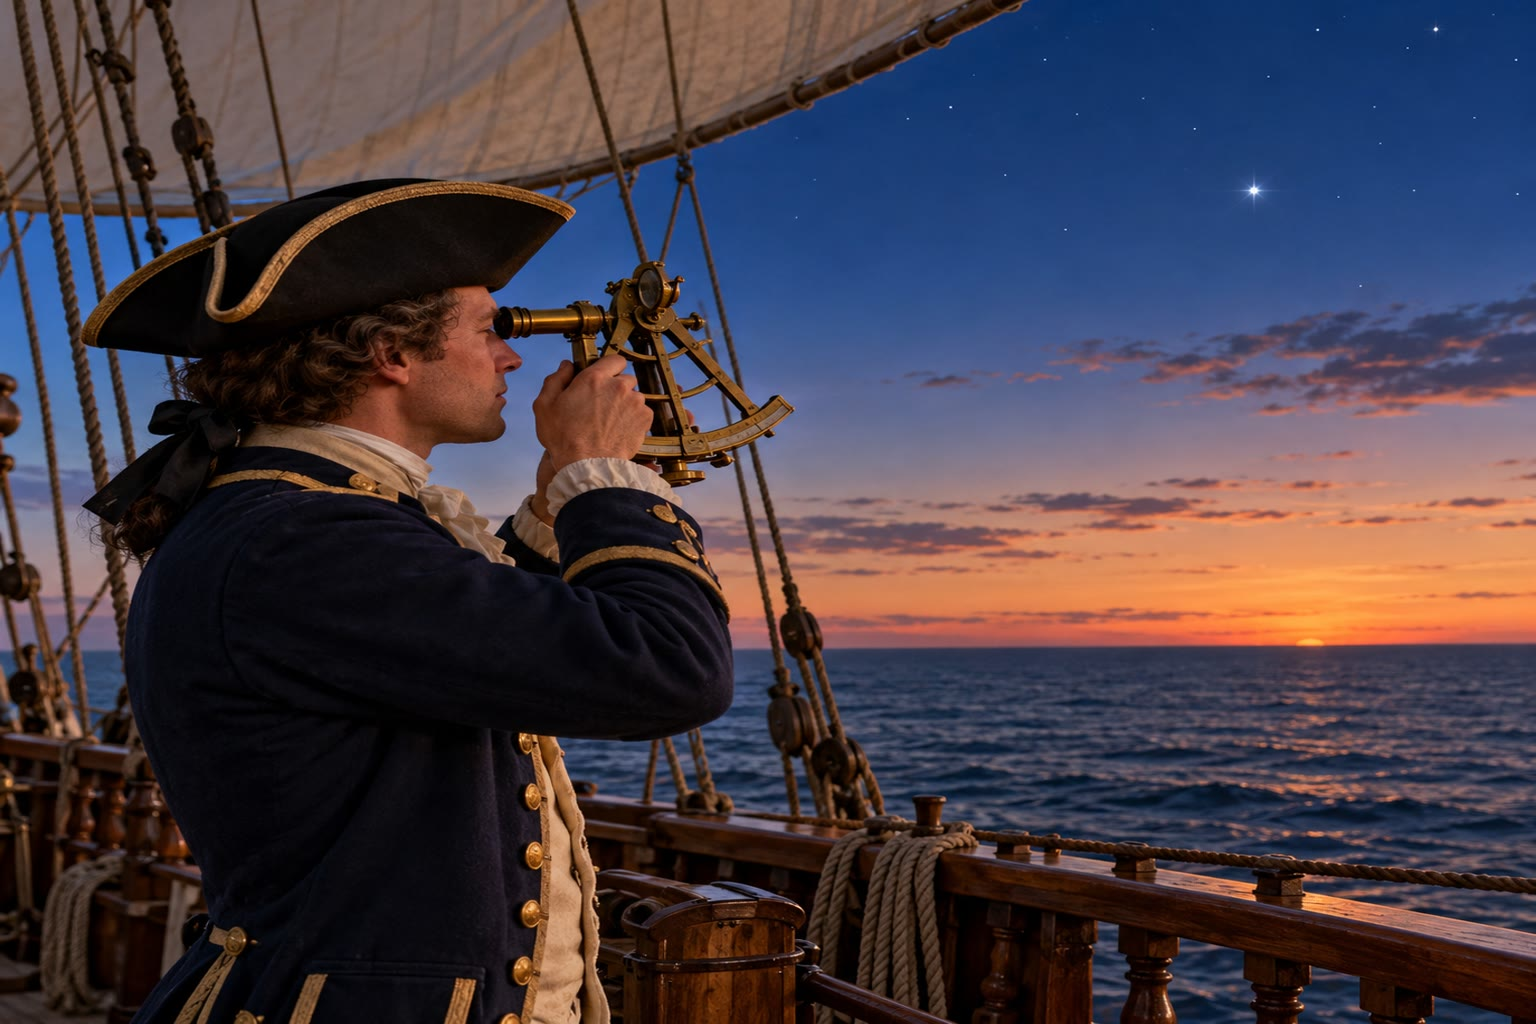
\includegraphics[width=0.62\linewidth]{images/book1/ai/g6-navigator-sextant.jpg}

{\small Un navigateur du \textsc{xviii}\textsuperscript{e}~siècle mesure la
hauteur d'une étoile au-dessus de l'horizon de la \omterm{def:g2:water-on-earth:ocean}{mer}. (Illustration
générée par IA.)}
\end{omfigure}

\begin{recall}
Un \omterm{def:g3:continents-and-oceans:globe}{globe} est une petite maquette de la Terre. L'\omterm{def:g3:continents-and-oceans:equator}{équateur} est la ligne qui
fait le tour du \omterm{def:g3:continents-and-oceans:globe}{globe} en son milieu, à mi-chemin entre le \omterm{def:g3:continents-and-oceans:poles}{pôle Nord} et le
\omterm{def:g3:continents-and-oceans:poles}{pôle Sud}~; il coupe la Terre en \omterm{def:g3:continents-and-oceans:equator}{hémisphère nord} et \omterm{def:g3:continents-and-oceans:equator}{hémisphère sud}
(\cref{ch:g3:continents-and-oceans}). Les livres de physique ont montré
que la Terre tourne sur elle-même autour d'un axe qui passe par les deux
\omterm{def:g3:continents-and-oceans:poles}{pôles}, une fois par jour~: cette rotation fait alterner le jour et la nuit.
\end{recall}

\section{Les parallèles et la latitude}

Pour dire où se trouve un lieu sur la Terre, il nous faut deux nombres,
comme le rang et la place d'un fauteuil au cinéma. Le premier indique à
quelle distance au nord ou au sud de l'\omterm{def:g3:continents-and-oceans:equator}{équateur} se trouve le lieu.

Imagine la Terre coupée en deux en passant par les deux \omterm{def:g3:continents-and-oceans:poles}{pôles}, comme une
pomme coupée depuis la queue vers le bas. Sur la face coupée (à gauche,
ci-dessous), l'\omterm{def:g3:continents-and-oceans:equator}{équateur} est la ligne horizontale qui passe par le centre.
Un lieu~P de la surface est vu depuis le centre sous un certain angle
au-dessus ou au-dessous de cette ligne~: cet angle est sa \omterm{def:g6:latitude-longitude:latitude}{latitude}.

\begin{omfigure}
\begin{minipage}[t]{0.48\linewidth}\centering
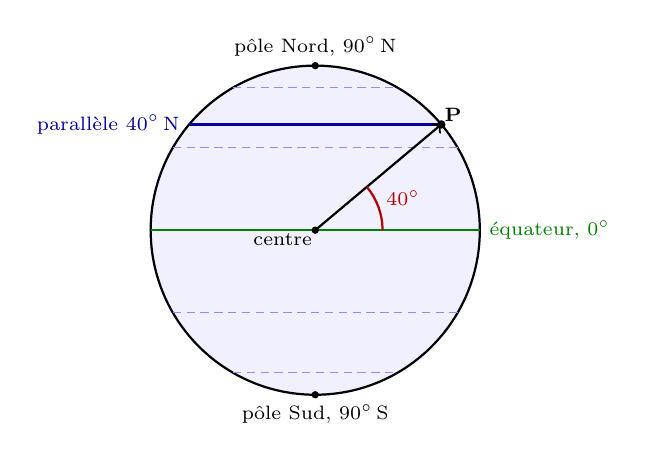
\begin{tikzpicture}[scale=0.95]
  \def\R{2.2}
  \fill[blue!6] (0,0) circle (\R);
  \draw[thick] (0,0) circle (\R);
  % parallels seen edge-on: horizontal chords
  \foreach \a in {-60,-30,30,60}{
    \draw[blue!45, densely dashed] ({-\R*cos(\a)},{\R*sin(\a)}) -- ({\R*cos(\a)},{\R*sin(\a)});}
    \draw[green!50!black, thick] (-\R,0) -- (\R,0);
  \node[font=\scriptsize, green!50!black, anchor=west] at (\R,0) {équateur, $0^\circ$};
  \draw[blue!60!black, thick] ({-\R*cos(40)},{\R*sin(40)}) -- ({\R*cos(40)},{\R*sin(40)});
  \draw[->, thick] (0,0) -- ({\R*cos(40)},{\R*sin(40)});
  \fill (0,0) circle (1.4pt) node[below left, font=\scriptsize, inner sep=1pt] {centre};
  \fill ({\R*cos(40)},{\R*sin(40)}) circle (1.6pt)
    node[above right, font=\scriptsize\bfseries, inner sep=1pt] {P};
  \draw[red!70!black, thick] (0.9,0) arc (0:40:0.9);
  \node[red!70!black, font=\scriptsize] at (20:1.25) {$40^\circ$};
  \node[font=\scriptsize, blue!60!black, anchor=east] at ({-\R*cos(40)},{\R*sin(40)}) {parallèle $40^\circ$\,N};
  \fill (0,\R) circle (1.4pt) node[above, font=\scriptsize] {pôle Nord, $90^\circ$\,N};
  \fill (0,-\R) circle (1.4pt) node[below, font=\scriptsize] {pôle Sud, $90^\circ$\,S};
\end{tikzpicture}

{\small La \omterm{def:g6:latitude-longitude:latitude}{latitude}~: l'angle, au centre de la Terre, entre l'\omterm{def:g3:continents-and-oceans:equator}{équateur} et
le lieu.}
\end{minipage}\hfill
\begin{minipage}[t]{0.48\linewidth}\centering
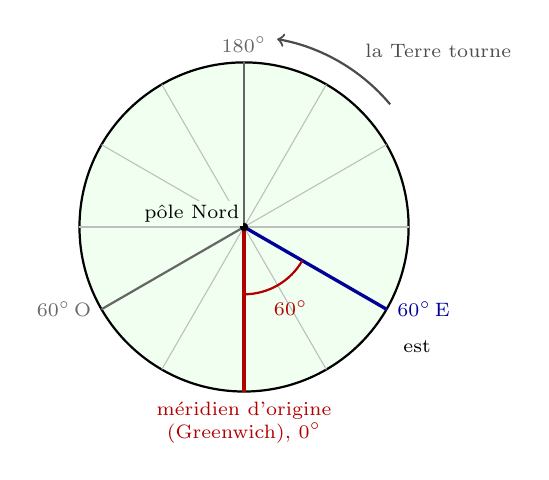
\begin{tikzpicture}[scale=0.95]
  \def\R{2.2}
  \fill[green!6] (0,0) circle (\R);
  \draw[thick] (0,0) circle (\R);
  \foreach \a in {0,30,...,330}{\draw[black!25] (0,0) -- (\a:\R);}
    \draw[red!70!black, very thick] (0,0) -- (270:\R)
    node[below, font=\scriptsize, align=center] {méridien d'origine\\(Greenwich), $0^\circ$};
  \draw[blue!60!black, very thick] (0,0) -- (330:\R)
    node[right, font=\scriptsize] {$60^\circ$\,E};
  \draw[black!60, thick] (0,0) -- (210:\R) node[left, font=\scriptsize] {$60^\circ$\,O};
  \draw[black!60, thick] (0,0) -- (90:\R) node[above, font=\scriptsize] {$180^\circ$};
  \draw[red!70!black, thick] (270:0.9) arc (270:330:0.9);
  \node[red!70!black, font=\scriptsize] at (300:1.25) {$60^\circ$};
    \fill (0,0) circle (1.6pt) node[above left, font=\scriptsize, inner sep=1.5pt, fill=green!6] {pôle Nord};
  \draw[->, thick, black!70] (40:2.55) arc (40:80:2.55);
  \node[font=\scriptsize, black!70, anchor=south west] at (55:2.6) {la Terre tourne};
  \node[font=\scriptsize, anchor=west] at (2.0,-1.6) {est $\circlearrowleft$};
\end{tikzpicture}

{\small La \omterm{def:g6:latitude-longitude:longitude}{longitude}~: la Terre vue au-dessus du \omterm{def:g3:continents-and-oceans:poles}{pôle Nord}. L'angle est
mesuré à partir du \omterm{def:g6:latitude-longitude:longitude}{méridien d'origine}, vers l'est ou vers l'ouest.}
\end{minipage}
% ledger: rmg:latitude-def, rmg:longitude-def
\end{omfigure}

\begin{definition}[Parallèle et latitude]\label{def:g6:latitude-longitude:latitude}
Un \emph{parallèle}\index{parallele@parallèle} est un cercle tracé autour
du \omterm{def:g3:continents-and-oceans:globe}{globe} parallèlement à l'\omterm{def:g3:continents-and-oceans:equator}{équateur}~; tous les lieux situés sur le même
parallèle sont à la même distance de l'\omterm{def:g3:continents-and-oceans:equator}{équateur}. La
\emph{latitude}\index{latitude} d'un lieu est l'angle, mesuré au centre de
la Terre, entre l'\omterm{def:g3:continents-and-oceans:equator}{équateur} et ce lieu. Elle va de $0^\circ$ à l'\omterm{def:g3:continents-and-oceans:equator}{équateur} à
$90^\circ$ aux \omterm{def:g3:continents-and-oceans:poles}{pôles}, et l'on précise si le lieu est au nord (N) ou au sud
(S) de l'\omterm{def:g3:continents-and-oceans:equator}{équateur}.
% ledger: rmg:latitude-def
\end{definition}

L'\omterm{def:g3:continents-and-oceans:equator}{équateur} est lui-même un \omterm{def:g6:latitude-longitude:latitude}{parallèle}, le plus long, de \omterm{def:g6:latitude-longitude:latitude}{latitude} $0^\circ$.
Les \omterm{def:g6:latitude-longitude:latitude}{parallèles} raccourcissent vers les \omterm{def:g3:continents-and-oceans:poles}{pôles}, et chaque \omterm{def:g3:continents-and-oceans:poles}{pôle} n'est qu'un
point, à $90^\circ$\,N ou à $90^\circ$\,S. Le long d'une ligne allant d'un
\omterm{def:g3:continents-and-oceans:poles}{pôle} à l'\omterm{def:g3:continents-and-oceans:equator}{équateur}, chaque degré de \omterm{def:g6:latitude-longitude:latitude}{latitude} mesure environ \qty{111}{km}.
% ledger: rmg:latitude-def

La \omterm{def:g6:latitude-longitude:latitude}{latitude} est le nombre facile~: on peut la trouver grâce au ciel. Le
jour, les marins mesuraient la hauteur du Soleil à midi~; la nuit, dans
l'\omterm{def:g3:continents-and-oceans:equator}{hémisphère nord}, ils mesuraient la hauteur de l'étoile Polaire. C'est ce
que fait le navigateur de l'image du début.
% ledger: rmg:15deg-per-hour

L'étoile Polaire se trouve presque exactement dans le prolongement de l'axe
de la Terre, au-delà du \omterm{def:g3:continents-and-oceans:poles}{pôle Nord}, et elle est si lointaine que sa lumière
atteint chaque lieu de la Terre selon des lignes parallèles. Au \omterm{def:g3:continents-and-oceans:poles}{pôle Nord},
elle est juste au-dessus de nos têtes, à $90^\circ$ au-dessus de
l'horizon~; à l'\omterm{def:g3:continents-and-oceans:equator}{équateur}, elle est posée sur l'horizon nord, à $0^\circ$.
Entre les deux, la règle est simple~:
\emph{la hauteur de l'étoile Polaire au-dessus de l'horizon nord, mesurée comme un angle, est égale à la \omterm{def:g6:latitude-longitude:latitude}{latitude}}.
La figure ci-dessous montre pourquoi les deux angles sont égaux.
% ledger: nsta:polaris-latitude

\begin{omfigure}
\begin{tikzpicture}[scale=1.1, font=\scriptsize]
  \def\R{1.7}
  \coordinate (O) at (0,0);
  \coordinate (P) at ({\R*cos(40)},{\R*sin(40)});
  \fill[blue!8] (O) circle (\R);
  \draw[black!70] (O) circle (\R);
  % equator and axis
  \draw[black!50] (-\R,0) -- (\R,0);
  \node[black!60, anchor=north east] at (-0.15,0) {équateur};
  \draw[black!70, -{Stealth[length=2mm]}] (0,-\R-0.3) -- (0,\R+1.7);
  \node[anchor=east, align=right] at (-0.1,\R+1.45) {vers l'étoile Polaire\\(très lointaine)};
  \node[anchor=south east] at (0,\R) {N};
  % radius to P and latitude angle at the centre
  \draw[black!80] (O) -- (P);
  \draw[red!70!black, thick] (0.55,0) arc (0:40:0.55);
  \node[red!70!black] at (20:0.8) {$40^\circ$};
  % horizon at P (tangent) and the ray to the Pole Star (parallel to the axis)
  \draw[black!70, thick] ($(P)+({-sin(40)*1.5},{cos(40)*1.5})$) -- ($(P)+({sin(40)*1.6},{-cos(40)*1.6})$);
  \node[anchor=south, rotate=-50, inner sep=2pt] at ($(P)+({sin(40)*1.15},{-cos(40)*1.15})$) {horizon};
  \draw[orange!80!black, thick, -{Stealth[length=2mm]}] (P) -- ++(0,1.45);
  \draw[red!70!black, thick] ($(P)+(0,0.7)$) arc (90:130:0.7);
  \node[red!70!black] at ($(P)+(110:0.98)$) {$40^\circ$};
  \fill (P) circle (1.4pt);
  \node[anchor=west] at ($(P)+(0.3,0.05)$) {observateur à $40^\circ$\,N};
\end{tikzpicture}

{\small Pourquoi la hauteur de l'étoile Polaire est égale à la \omterm{def:g6:latitude-longitude:latitude}{latitude}
(croquis, pas à l'échelle). La lumière de l'étoile Polaire arrive
parallèlement à l'axe de la Terre (en orange). L'horizon de l'observateur
est perpendiculaire au rayon qui passe par l'observateur~; l'axe est
perpendiculaire à l'\omterm{def:g3:continents-and-oceans:equator}{équateur}. L'angle entre l'horizon et l'étoile Polaire
est donc égal à la \omterm{def:g6:latitude-longitude:latitude}{latitude}, l'angle au centre entre l'\omterm{def:g3:continents-and-oceans:equator}{équateur} et
l'observateur.}
% ledger: nsta:polaris-latitude
\end{omfigure}

\begin{example}[Une navigatrice dans la nuit]\label{ex:g6:latitude-longitude:pole-star}
Une navigatrice mesure l'étoile Polaire à $41^\circ$ au-dessus de l'horizon
nord. Le navire est à la \omterm{def:g6:latitude-longitude:latitude}{latitude} $41^\circ$\,N, à environ $41 \times 111
\approx \num{4550}$~km au nord de l'\omterm{def:g3:continents-and-oceans:equator}{équateur}. En naviguant vers le nord,
elle trouve l'étoile un peu plus haute chaque nuit~; en naviguant vers le
sud, vers l'\omterm{def:g3:continents-and-oceans:equator}{équateur}, l'étoile descend vers l'horizon. Au sud de
l'\omterm{def:g3:continents-and-oceans:equator}{équateur}, l'étoile Polaire est invisible, car elle reste sous
l'horizon~: là, c'est le Soleil de midi qui donne la \omterm{def:g6:latitude-longitude:latitude}{latitude}.
\end{example}
% ledger: nsta:polaris-latitude, rmg:latitude-def, rmg:15deg-per-hour

\section{Les méridiens et la longitude}

Le second nombre indique à quelle distance vers l'est ou vers l'ouest se
trouve un lieu. Ici, il n'y a pas de ligne de départ naturelle comme
l'\omterm{def:g3:continents-and-oceans:equator}{équateur}~: il faut en choisir une.

\begin{definition}[Méridien, longitude et méridien d'origine]\label{def:g6:latitude-longitude:longitude}
Un \emph{méridien}\index{meridien@méridien} est un demi-cercle tracé sur
le \omterm{def:g3:continents-and-oceans:globe}{globe} du \omterm{def:g3:continents-and-oceans:poles}{pôle Nord} au \omterm{def:g3:continents-and-oceans:poles}{pôle Sud}. Le
\emph{méridien d'origine}\index{meridien d'origine@méridien d'origine} est
le méridien choisi comme ligne de départ~: celui qui passe par l'ancien
Observatoire royal de Greenwich, à Londres. La
\emph{longitude}\index{longitude} d'un lieu est l'angle entre le méridien
d'origine et le méridien de ce lieu, vu depuis l'axe de la Terre. Elle va
de $0^\circ$ au méridien d'origine à $180^\circ$, et l'on précise si le
lieu est à l'est (E) ou à l'ouest (O) du méridien d'origine.
% ledger: rmg:longitude-def
\end{definition}

Tous les \omterm{def:g6:latitude-longitude:longitude}{méridiens} se rejoignent aux \omterm{def:g3:continents-and-oceans:poles}{pôles}, et ils ont tous la même
longueur. Du côté de la Terre opposé à Greenwich, le \omterm{def:g6:latitude-longitude:longitude}{méridien}
$180^\circ$\,E et le \omterm{def:g6:latitude-longitude:longitude}{méridien} $180^\circ$\,O sont la même ligne.

\begin{omfigure}
\begin{minipage}[c]{0.46\linewidth}\centering
\begin{tikzpicture}
  \begin{axis}[axis equal image, hide axis, width=\linewidth,
      xmin=-1.05, xmax=1.05, ymin=-1.05, ymax=1.12, clip=false]
    \fill[omSea] (axis cs:0,0) circle (1);
    \addplot[fill=omLithAlluv, draw=black!45, line width=0.2pt] table {figdata/out/grade-6-graticule-land.dat};
    \addplot[blue!50!black, line width=0.35pt] table {figdata/out/grade-6-graticule-parallels.dat};
    \addplot[black!55, line width=0.35pt] table {figdata/out/grade-6-graticule-meridians.dat};
        \addplot[green!50!black, line width=1.1pt] table {figdata/out/grade-6-graticule-equator.dat};
    \addplot[red!70!black, line width=1.1pt] table {figdata/out/grade-6-graticule-prime.dat};
    \draw[black!70] (axis cs:0,0) circle (1);
    \fill (axis cs:0,0.9063) circle (1.3pt);
        \node[font=\scriptsize, above left, inner sep=1.5pt] at (axis cs:0,0.9063) {N};
  \end{axis}
\end{tikzpicture}
\end{minipage}\hfill
\begin{minipage}[c]{0.5\linewidth}
{\small Un \omterm{def:g3:continents-and-oceans:globe}{globe} avec ses \omterm{def:g6:latitude-longitude:latitude}{parallèles} (en bleu) et ses \omterm{def:g6:latitude-longitude:longitude}{méridiens} (en gris),
tous les $30^\circ$. L'\omterm{def:g3:continents-and-oceans:equator}{équateur} est tracé en vert épais, le \omterm{def:g6:latitude-longitude:longitude}{méridien
d'origine} en rouge~; ils se croisent dans l'\omterm{def:g2:water-on-earth:ocean}{océan}, au sud du Ghana, à la
\omterm{def:g6:latitude-longitude:latitude}{latitude} $0^\circ$ et à la \omterm{def:g6:latitude-longitude:longitude}{longitude} $0^\circ$. Chaque \omterm{def:g6:latitude-longitude:longitude}{méridien} va d'un
\omterm{def:g3:continents-and-oceans:poles}{pôle} à l'autre~; chaque \omterm{def:g6:latitude-longitude:latitude}{parallèle} est un cercle autour de l'axe. (Terres~:
Natural Earth.)}
% ledger: data:ne-land (figdata/grade-6/graticule.py)
\end{minipage}
\end{omfigure}

\begin{history}[Le choix du méridien d'origine]
Pendant longtemps, chaque pays a dessiné ses \omterm{def:g2:drawing-to-map:map}{cartes} avec son propre
\omterm{def:g6:latitude-longitude:longitude}{méridien} de départ~: Londres, Paris et d'autres lieux ont tous servi. En
octobre 1884, des délégués de nombreux pays se sont réunis à Washington
pour choisir un seul \omterm{def:g6:latitude-longitude:longitude}{méridien} pour le monde entier. Le 13~octobre, ils ont
voté pour proposer le \omterm{def:g6:latitude-longitude:longitude}{méridien} qui passe par l'observatoire de
Greenwich~: 21 pays ont voté pour, un contre, et deux n'ont pas pris part
au vote.
% ledger: rmg:longitude-def, meridian:1884-vote
\end{history}

\section{Trouver un lieu grâce à ses deux angles}

Avec sa \omterm{def:g6:latitude-longitude:latitude}{latitude} et sa \omterm{def:g6:latitude-longitude:longitude}{longitude}, on peut trouver n'importe quel lieu de la
Terre, sur une \omterm{def:g2:drawing-to-map:map}{carte} ou sur un \omterm{def:g3:continents-and-oceans:globe}{globe}. On écrit d'abord la \omterm{def:g6:latitude-longitude:latitude}{latitude}~: Le
Caire, par exemple, est à environ $30^\circ$\,N, $31^\circ$\,E.
% ledger: data:b1-ne-places (figdata/grade-6/cities.py)

\begin{omfigure}
\begin{tikzpicture}
  \begin{axis}[ommap, width=\linewidth,
      xtick={-180,-150,...,180}, ytick={-90,-60,...,90},
      xticklabels={$180^\circ$,$150^\circ$O,$120^\circ$O,$90^\circ$O,$60^\circ$O,$30^\circ$O,$0^\circ$,
                   $30^\circ$E,$60^\circ$E,$90^\circ$E,$120^\circ$E,$150^\circ$E,$180^\circ$},
      yticklabels={$90^\circ$S,$60^\circ$S,$30^\circ$S,$0^\circ$,$30^\circ$N,$60^\circ$N,$90^\circ$N},
      tick label style={font=\tiny}, grid style={black!35, line width=0.3pt}]
    \addplot[fill=omLithAlluv, draw=black!45, line width=0.2pt] table {figdata/out/shared-geo-land.dat};
        \draw[green!50!black, line width=0.9pt] (axis cs:-180,0) -- (axis cs:180,0);
    \draw[red!70!black, line width=0.9pt] (axis cs:0,-90) -- (axis cs:0,90);
    \addplot[only marks, mark=*, mark size=1.2pt, black]
      table[x=lon, y=lat] {figdata/out/grade-6-cities-map.dat};
    \node[font=\tiny, inner sep=1.2pt, fill=white, fill opacity=0.75, text opacity=1, anchor=south] at (axis cs:-21.936,64.144) {Reykjavík};
    \node[font=\tiny, inner sep=1.2pt, fill=white, fill opacity=0.75, text opacity=1, anchor=south] at (axis cs:-0.119,51.502) {Londres};
    \node[font=\tiny, inner sep=1.2pt, fill=white, fill opacity=0.75, text opacity=1, anchor=west] at (axis cs:-73.996,40.722) {New~York};
    \node[font=\tiny, inner sep=1.2pt, fill=white, fill opacity=0.75, text opacity=1, anchor=east] at (axis cs:-118.232,34.049) {Los~Angeles};
    \node[font=\tiny, inner sep=1.2pt, fill=white, fill opacity=0.75, text opacity=1, anchor=east] at (axis cs:-78.502,-0.213) {Quito};
    \node[font=\tiny, inner sep=1.2pt, fill=white, fill opacity=0.75, text opacity=1, anchor=west] at (axis cs:-43.212,-22.907) {Rio~de~Janeiro};
    \node[font=\tiny, inner sep=1.2pt, fill=white, fill opacity=0.75, text opacity=1, anchor=north] at (axis cs:18.433,-33.918) {Le~Cap};
    \node[font=\tiny, inner sep=1.2pt, fill=white, fill opacity=0.75, text opacity=1, anchor=west] at (axis cs:36.815,-1.281) {Nairobi};
    \node[font=\tiny, inner sep=1.2pt, fill=white, fill opacity=0.75, text opacity=1, anchor=south] at (axis cs:31.248,30.052) {Le~Caire};
    \node[font=\tiny, inner sep=1.2pt, fill=white, fill opacity=0.75, text opacity=1, anchor=north] at (axis cs:72.876,19.068) {Bombay};
    \node[font=\tiny, inner sep=1.2pt, fill=white, fill opacity=0.75, text opacity=1, anchor=west] at (axis cs:139.75,35.687) {Tokyo};
    \node[font=\tiny, inner sep=1.2pt, fill=white, fill opacity=0.75, text opacity=1, anchor=south] at (axis cs:151.213,-33.871) {Sydney};
    \node[font=\tiny, inner sep=1.2pt, fill=white, fill opacity=0.75, text opacity=1, anchor=north east] at (axis cs:174.763,-36.848) {Auckland};
  \end{axis}
\end{tikzpicture}

{\small Treize villes sur une \omterm{def:g2:drawing-to-map:map}{carte} du monde, avec un quadrillage tous les
$30^\circ$. L'\omterm{def:g3:continents-and-oceans:equator}{équateur} est tracé en vert, le \omterm{def:g6:latitude-longitude:longitude}{méridien d'origine} en rouge.
(Côtes et villes~: Natural Earth.)}
% ledger: data:ne-land, data:b1-ne-places (figdata/grade-6/cities.py, part map)
\end{omfigure}

\begin{method}[Repérer un lieu par ses coordonnées]\label{met:g6:latitude-longitude:locating}
\begin{enumerate}
  \item \omterm{def:g6:latitude-longitude:latitude}{Latitude}~: pars de l'\omterm{def:g3:continents-and-oceans:equator}{équateur} et va vers le nord (N) ou vers le sud
        (S), en comptant les \omterm{def:g6:latitude-longitude:latitude}{parallèles}, jusqu'au bon nombre de degrés.
  \item \omterm{def:g6:latitude-longitude:longitude}{Longitude}~: pars du \omterm{def:g6:latitude-longitude:longitude}{méridien d'origine} et va vers l'est (E) ou vers
        l'ouest (O), en comptant les \omterm{def:g6:latitude-longitude:longitude}{méridiens}, jusqu'au bon nombre de
        degrés.
  \item Le lieu se trouve là où le \omterm{def:g6:latitude-longitude:latitude}{parallèle} et le \omterm{def:g6:latitude-longitude:longitude}{méridien} se croisent.
        Entre deux lignes du quadrillage, estime~: à mi-chemin entre
        $30^\circ$ et $60^\circ$, on est à $45^\circ$.
\end{enumerate}
\end{method}

\begin{example}[Lire les coordonnées de Sydney]\label{ex:g6:latitude-longitude:sydney}
Sur la \omterm{def:g2:drawing-to-map:map}{carte}, Sydney se trouve sous l'\omterm{def:g3:continents-and-oceans:equator}{équateur}~: elle est dans
l'\omterm{def:g3:continents-and-oceans:equator}{hémisphère sud}, un peu au-dessus du \omterm{def:g6:latitude-longitude:latitude}{parallèle} $30^\circ$\,S, plus près
de $30^\circ$ que de $60^\circ$~; sa \omterm{def:g6:latitude-longitude:latitude}{latitude} est d'environ $34^\circ$\,S.
Elle se trouve à droite du \omterm{def:g6:latitude-longitude:longitude}{méridien d'origine}, un peu au-delà du \omterm{def:g6:latitude-longitude:longitude}{méridien}
$150^\circ$\,E~; sa \omterm{def:g6:latitude-longitude:longitude}{longitude} est d'environ $151^\circ$\,E. On écrit~:
Sydney, $34^\circ$\,S, $151^\circ$\,E.
% ledger: data:b1-ne-places (cities.py: 33.87 S, 151.21 E)
\end{example}

\section{La Terre qui tourne et les fuseaux horaires}

La Terre tourne sur elle-même une fois par jour, d'ouest en est. Pendant
qu'elle tourne, le Soleil semble traverser le ciel d'est en ouest. Quand le
Soleil est au plus haut dans le ciel, il est midi. Mais il n'est pas midi
partout au même moment~: quand il est midi à Londres, c'est déjà
l'après-midi au Caire, plus à l'est, et c'est encore le matin à New York,
plus à l'ouest.

De combien la Terre tourne-t-elle en une heure~? Un tour complet fait
$360^\circ$, et il dure 24~heures~:
\[
360^\circ \div 24 = 15^\circ \text{ par heure.}
\]
Deux lieux distants de $15^\circ$ de \omterm{def:g6:latitude-longitude:longitude}{longitude} ont donc leur midi à une
heure d'intervalle~: le lieu situé le plus à l'est l'a en premier. Un degré
prend 4~minutes.
% ledger: planet:Earth.day, rmg:15deg-per-hour

\begin{definition}[Fuseau horaire]\label{def:g6:latitude-longitude:time-zone}
Un \emph{fuseau horaire}\index{fuseau horaire} est une bande de la Terre,
d'un \omterm{def:g3:continents-and-oceans:poles}{pôle} à l'autre, où toutes les horloges indiquent la même heure. Dans
l'idéal, chaque fuseau a une largeur de $15^\circ$ de \omterm{def:g6:latitude-longitude:longitude}{longitude}, si bien
qu'il y a 24 fuseaux, un par heure~; quand on passe d'un fuseau à celui
qui est à l'est, les horloges indiquent une heure de plus.
\end{definition}

Dans les fuseaux idéaux, le fuseau d'un lieu est sa \omterm{def:g6:latitude-longitude:longitude}{longitude} divisée par
$15$, arrondie à l'unité~: à l'est de Greenwich, on ajoute ce nombre
d'heures à l'heure de Greenwich~; à l'ouest, on le retranche. Tokyo, à
$140^\circ$\,E~: $140 \div 15 \approx 9.3$, donc le fuseau est $+9$~:
quand il est midi à Greenwich, il est 21~h à Tokyo. Les vrais fuseaux
horaires ne sont pas des bandes droites~: ils suivent les frontières des
pays et des régions, pour qu'un pays entier, ou une région entière, garde
la même heure.
% ledger: data:b1-ne-places, rmg:15deg-per-hour

\begin{omfigure}
\begin{tikzpicture}
  \begin{axis}[ommap, width=\linewidth, clip=false,
      xtick={-180,-90,0,90,180}, ytick={-60,0,60},
      xticklabels={$180^\circ$,$90^\circ$O,$0^\circ$,$90^\circ$E,$180^\circ$},
      yticklabels={$60^\circ$S,$0^\circ$,$60^\circ$N},
      tick label style={font=\tiny}, grid=none]
    \addplot[fill=black!8, draw=none] table {figdata/out/grade-6-time_zones-odd.dat};
    \addplot[fill=omLithAlluv, fill opacity=0.85, draw=black!45, line width=0.2pt] table {figdata/out/shared-geo-land.dat};
    \addplot[only marks, mark=none, point meta=explicit symbolic,
        nodes near coords, nodes near coords style={font=\tiny, anchor=south, inner sep=1pt}]
            table[x=lon, y=y, meta=label] {figdata/out/grade-6-time_zones-labels.dat};
    \draw[red!75!black, line width=1.6pt] (axis cs:180,-90) -- (axis cs:180,90);
    \draw[red!75!black, line width=1.6pt] (axis cs:-180,-90) -- (axis cs:-180,90);
        \draw[black, line width=0.8pt] (axis cs:0,-90) -- (axis cs:0,90);
    \node[font=\scriptsize, red!75!black, rotate=90, anchor=south] at (axis cs:180,0) {changement de date};
    \node[font=\scriptsize, red!75!black, rotate=90, anchor=north] at (axis cs:-180,0) {changement de date};
  \end{axis}
\end{tikzpicture}

{\small Les 24 fuseaux horaires idéaux, larges chacun de $15^\circ$, avec le
nombre d'heures à ajouter à l'heure de Greenwich (la ligne noire au
milieu). La \omterm{def:g6:latitude-longitude:date-line}{ligne de changement de date} suit le \omterm{def:g6:latitude-longitude:longitude}{méridien} $180^\circ$, que
cette \omterm{def:g2:drawing-to-map:map}{carte} coupe en deux~: il forme à la fois le bord gauche et le bord
droit. Roule la \omterm{def:g2:drawing-to-map:map}{carte} en tube, et les deux lignes rouges n'en font plus
qu'une. Le fuseau situé de chaque côté de la \omterm{def:g6:latitude-longitude:date-line}{ligne de changement de date}
n'a qu'une demi-largeur.}
% ledger: rmg:15deg-per-hour, planet:Earth.day (figdata/grade-6/time_zones.py)
\end{omfigure}

\paragraph{La ligne de changement de date.} Pars de Greenwich vers l'est,
en ajoutant une heure par fuseau~: à $180^\circ$, tu as 12~heures d'avance.
Pars vers l'ouest, en retranchant une heure par fuseau~: à $180^\circ$, tu
as 12~heures de retard. Les deux voyageurs se retrouvent sur le même
\omterm{def:g6:latitude-longitude:longitude}{méridien}, avec des horloges qui indiquent la même heure, mais à un jour
entier d'écart~! L'un d'eux doit changer de date.

\begin{definition}[Ligne internationale de changement de date]\label{def:g6:latitude-longitude:date-line}
La \emph{ligne de changement de date}\index{ligne de changement de date} est
la ligne, au milieu de l'\omterm{def:g2:water-on-earth:ocean}{océan} Pacifique, où la date change. Elle suit le
\omterm{def:g6:latitude-longitude:longitude}{méridien} $180^\circ$, avec quelques détours pour ne pas couper un pays en
deux. En la traversant vers l'ouest, on passe au jour suivant~; en la
traversant vers l'est, on revient au jour précédent.
\end{definition}

\begin{history}[La montre de marine de Harrison]
\begin{minipage}[c]{0.7\linewidth}
Pour trouver sa \omterm{def:g6:latitude-longitude:longitude}{longitude}, un navigateur compare deux heures~: l'heure
locale du navire, lue sur le Soleil, et, au même moment, l'heure de son
port d'attache. Chaque heure d'écart représente $15^\circ$ de \omterm{def:g6:latitude-longitude:longitude}{longitude}. La
difficulté était de transporter l'heure du port à travers l'\omterm{def:g2:water-on-earth:ocean}{océan}~: même
les meilleures montres de l'époque n'étaient pas assez précises.
L'horloger anglais John Harrison a consacré des dizaines d'années à ce
problème, en visant une horloge qui ne prendrait ni ne perdrait plus de
3~secondes par jour. Son quatrième garde-temps de marine, appelé H4,
ressemble à une grosse montre de poche et fait tic-tac cinq fois par
seconde. En 1761, son fils William l'a emporté lors d'un voyage vers la
Jamaïque pour l'essayer.
% ledger: rmg:15deg-per-hour, rmg:longitude-act-1714, rmg:h4-jamaica-1761
\end{minipage}\hfill
\begin{minipage}[c]{0.26\linewidth}\centering
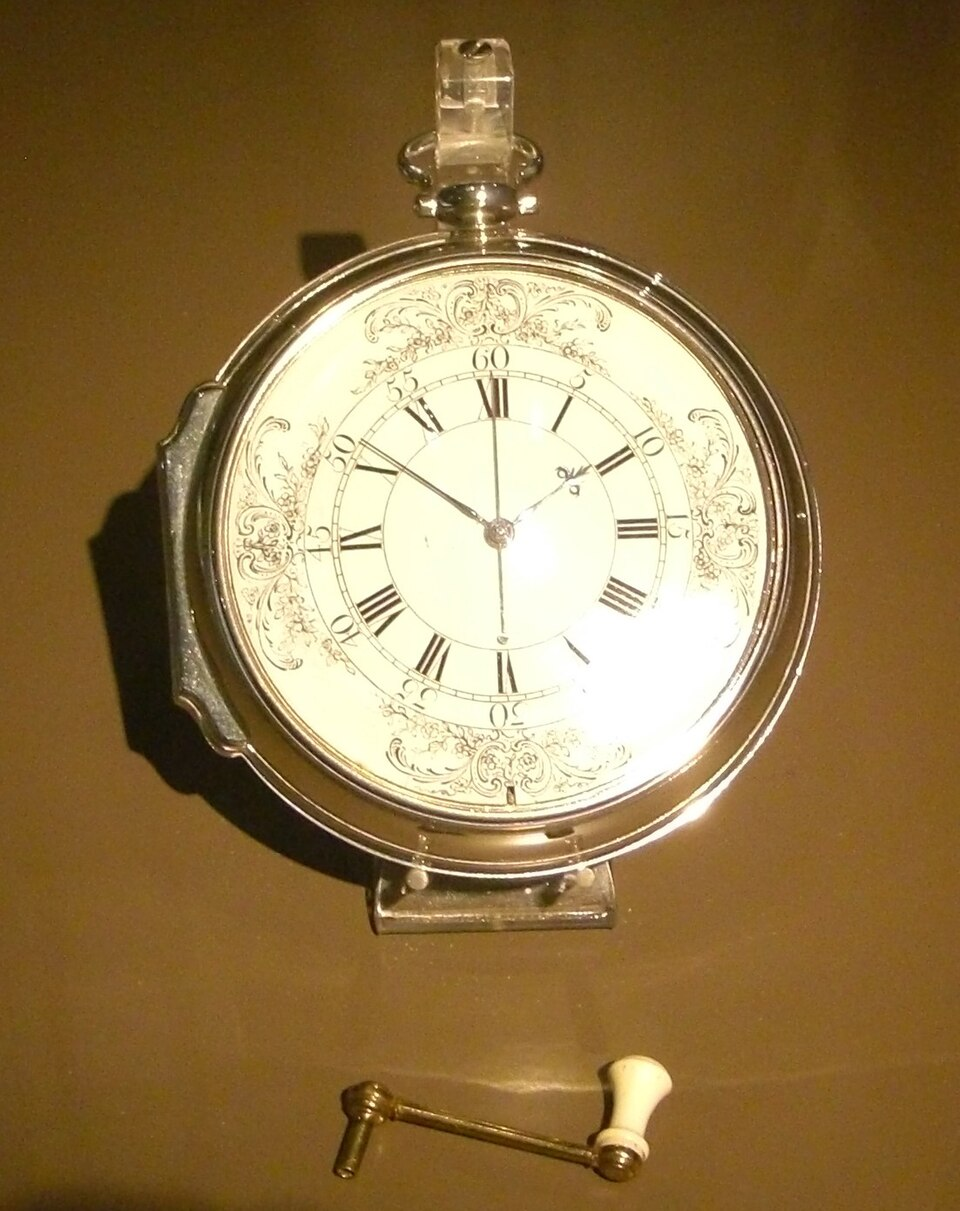
\includegraphics[width=\linewidth]{images/book1/g6-harrison-h4.jpg}\\[2pt]
{\footnotesize Le H4 de Harrison, National Maritime Museum, Greenwich.
(Photo~: Colonel Warden, CC BY-SA 3.0, via Wikimedia Commons.)}
% ledger: commons:harrison-h4
\end{minipage}
\end{history}

\section{Exercices}

\begin{exercise}[$\star$]\label{exo:g6:latitude-longitude:1}
Recopie et complète~: «~La \omterm{def:g6:latitude-longitude:latitude}{latitude} se mesure à partir de l'\ldots{} et va
de $0^\circ$ à \ldots~; la \omterm{def:g6:latitude-longitude:longitude}{longitude} se mesure à partir du \omterm{def:g6:latitude-longitude:longitude}{méridien}
d'\ldots{} et va de $0^\circ$ à \ldots~»
\end{exercise}

\begin{exercise}[$\star$]\label{exo:g6:latitude-longitude:2}
Quelle est la \omterm{def:g6:latitude-longitude:latitude}{latitude} du \omterm{def:g3:continents-and-oceans:poles}{pôle Nord}~? Du \omterm{def:g3:continents-and-oceans:poles}{pôle Sud}~? D'une ville située sur
l'\omterm{def:g3:continents-and-oceans:equator}{équateur}~?
\end{exercise}

\begin{exercise}[$\star$]\label{exo:g6:latitude-longitude:3}
À l'aide de la \omterm{def:g2:drawing-to-map:map}{carte} des treize villes, dis dans quel \omterm{def:g3:continents-and-oceans:equator}{hémisphère}, nord ou
sud, et de quel côté du \omterm{def:g6:latitude-longitude:longitude}{méridien d'origine}, est ou ouest, se trouve chacune
de ces villes~: Sydney, New York, Le Caire, Rio de Janeiro.
\end{exercise}

\begin{exercise}[$\star$]\label{exo:g6:latitude-longitude:4}
Vrai ou faux~? Corrige les phrases fausses.
(a) Tous les \omterm{def:g6:latitude-longitude:longitude}{méridiens} se rejoignent aux \omterm{def:g3:continents-and-oceans:poles}{pôles}.
(b) Tous les \omterm{def:g6:latitude-longitude:latitude}{parallèles} ont la même longueur.
(c) L'\omterm{def:g3:continents-and-oceans:equator}{équateur} est un \omterm{def:g6:latitude-longitude:latitude}{parallèle}.
(d) Le \omterm{def:g6:latitude-longitude:longitude}{méridien d'origine} passe par Paris.
\end{exercise}

\begin{exercise}[$\star\star$]\label{exo:g6:latitude-longitude:5}
À l'aide de la \omterm{def:g2:drawing-to-map:map}{carte} des treize villes, quelle ville se trouve à environ
$30^\circ$\,N, $31^\circ$\,E~? Laquelle à environ $41^\circ$\,N,
$74^\circ$\,O~? Donne les coordonnées approximatives de Tokyo.
% ledger: data:b1-ne-places (cities.py main table)
\end{exercise}

\begin{exercise}[$\star\star$]\label{exo:g6:latitude-longitude:6}
La ville~A est à la \omterm{def:g6:latitude-longitude:longitude}{longitude} $0^\circ$ et la ville~B à la \omterm{def:g6:latitude-longitude:longitude}{longitude}
$45^\circ$\,E. Combien d'heures séparent leurs midis~? Dans quelle ville
est-il midi en premier~?
\end{exercise}

\begin{exercise}[$\star\star$]\label{exo:g6:latitude-longitude:7}
Bombay est à environ $73^\circ$\,E. Calcule son \omterm{def:g6:latitude-longitude:time-zone}{fuseau horaire} idéal.
Quand il est midi à Greenwich, quelle heure est-il à Bombay, dans les
fuseaux idéaux~?
% ledger: data:b1-ne-places (cities.py: 72.88 E, zone +5)
\end{exercise}

\begin{exercise}[$\star\star$]\label{exo:g6:latitude-longitude:8}
Chaque degré de \omterm{def:g6:latitude-longitude:latitude}{latitude} mesure environ \qty{111}{km}. À quelle distance
de l'\omterm{def:g3:continents-and-oceans:equator}{équateur} se trouve une ville située à $30^\circ$\,N, mesurée le long
de son \omterm{def:g6:latitude-longitude:longitude}{méridien}~? À quelle distance de l'\omterm{def:g3:continents-and-oceans:equator}{équateur} se trouve le \omterm{def:g3:continents-and-oceans:poles}{pôle Nord}~?
% ledger: rmg:latitude-def
\end{exercise}

\begin{exercise}[$\star\star$]\label{exo:g6:latitude-longitude:9}
New York est dans le fuseau $-5$ et Tokyo dans le fuseau $+9$. Combien
d'heures séparent leurs horloges~? Quand il est 8~h le lundi à New York,
quelle heure et quel jour est-il à Tokyo~?
% ledger: data:b1-ne-places (cities.py: zones -5 and +9)
\end{exercise}

\begin{exercise}[$\star\star$]\label{exo:g6:latitude-longitude:10}
Lena dit~: «~Le Soleil se lève à l'est, donc les villes de l'est voient le
Soleil se lever avant les villes de l'ouest.~» A-t-elle raison~? Explique
à l'aide de la rotation de la Terre.
\end{exercise}

\begin{exercise}[$\star\star\star$]\label{exo:g6:latitude-longitude:11}
L'horloge d'un navire avance de 3~secondes par jour (elle va trop vite).
(a) De combien de secondes avance-t-elle après un voyage de 42~jours~?
(b) La Terre tourne d'un degré en 4~minutes, soit 240~secondes. Quelle
erreur, en degrés de \omterm{def:g6:latitude-longitude:longitude}{longitude}, l'erreur de l'horloge entraîne-t-elle~?
(c) À l'\omterm{def:g3:continents-and-oceans:equator}{équateur}, un degré de \omterm{def:g6:latitude-longitude:longitude}{longitude} mesure environ \qty{111}{km}. De
combien de kilomètres environ le navigateur se trompe-t-il, à l'\omterm{def:g3:continents-and-oceans:equator}{équateur}~?
% ledger: rmg:longitude-act-1714, rmg:15deg-per-hour, rmg:latitude-def
\end{exercise}

\begin{exercise}[$\star\star\star$]\label{exo:g6:latitude-longitude:12}
Un avion quitte Tokyo (fuseau $+9$) le lundi à 18~h et vole vers l'est, à
travers le Pacifique, jusqu'à Los Angeles (fuseau $-8$). Le vol dure
10~heures. (a) Quelle heure est-il à Greenwich quand l'avion décolle~?
(b) Quelle heure est-il à Greenwich quand il atterrit~? (c) Quels sont
l'heure locale et le jour à Los Angeles quand il atterrit~? Pourquoi les
voyageurs disent-ils que, sur ce vol, «~on atterrit avant d'avoir
décollé~»~?
\end{exercise}

\section{Problème~: Un appel vidéo autour du monde}

\begin{problem}[{Problème du week-end --- cinq amis, quatre fuseaux horaires et une
ligne de changement de date~: quelle heure est-il à Auckland quand l'appel commence~?}]
\label{pb:g6:latitude-longitude:1}
% ledger: data:b1-ne-places, rmg:15deg-per-hour, planet:Earth.day (cities.py, time_zones.py; test_cities_zones_used_in_the_problem)
Lena habite à Londres. Elle veut organiser un appel vidéo avec quatre amis
rencontrés en vacances~: Ana à Rio de Janeiro, Kenji à Tokyo, Mia à
Auckland et Sam à Los Angeles. Dans ce problème, nous utilisons les fuseaux
horaires idéaux.

\begin{center}
\small
\begin{tabular}{lll}
\hline
ami & ville & coordonnées\\
\hline
Lena & Londres & $52^\circ$\,N, $0^\circ$\\
Ana & Rio de Janeiro & $23^\circ$\,S, $43^\circ$\,O\\
Kenji & Tokyo & $36^\circ$\,N, $140^\circ$\,E\\
Mia & Auckland & $37^\circ$\,S, $175^\circ$\,E\\
Sam & Los Angeles & $34^\circ$\,N, $118^\circ$\,O\\
\hline
\end{tabular}
\end{center}

\medskip
\noindent\textbf{Partie I --- Où vivent les amis.}
\begin{enumerate}
  \item Quels amis vivent dans l'\omterm{def:g3:continents-and-oceans:equator}{hémisphère sud}~?
  \item Quels amis vivent à l'ouest du \omterm{def:g6:latitude-longitude:longitude}{méridien d'origine}~?
  \item Quel ami vit le plus loin de l'\omterm{def:g3:continents-and-oceans:equator}{équateur}~?
  \item Quel ami vit le plus près du \omterm{def:g6:latitude-longitude:longitude}{méridien} $180^\circ$~? À combien de
        degrés de \omterm{def:g6:latitude-longitude:longitude}{longitude} de celui-ci~?
\end{enumerate}

\medskip
\noindent\textbf{Partie II --- Quelle heure est-il~?}
\begin{enumerate}[resume]
  \item De combien de degrés la Terre tourne-t-elle en une heure~?
  \item Calcule le \omterm{def:g6:latitude-longitude:time-zone}{fuseau horaire} idéal de la ville de chaque ami.
  \item Lena propose de commencer l'appel le vendredi à 20~h, heure de
        Londres. Quels sont alors l'heure et le jour à Rio de Janeiro~? À
        Tokyo~?
  \item Kenji répond qu'il dormira. Explique pourquoi il est déjà samedi à
        Tokyo.
\end{enumerate}

\medskip
\noindent\textbf{Partie III --- Traverser la ligne de changement de date.}
\begin{enumerate}[resume]
  \item Quels sont l'heure et le jour à Los Angeles quand l'appel
        commence~?
  \item De combien d'heures les horloges d'Auckland sont-elles en avance
        sur celles de Los Angeles~?
  \item En naviguant vers l'est, d'Auckland à Los Angeles, un navire
        traverse la \omterm{def:g6:latitude-longitude:date-line}{ligne de changement de date}. Passe-t-il au jour suivant
        ou revient-il au jour précédent~?
  \item Quels sont l'heure locale et le jour à Auckland quand l'appel
        commence~?
\end{enumerate}
\end{problem}
